\documentclass[11pt]{article}
\usepackage[utf8]{inputenc}
\usepackage{fancyhdr}
\usepackage{diagbox}
\usepackage[english]{babel}
\usepackage{latexsym}
\usepackage{graphicx}
\usepackage{subfigure}
\usepackage{array}
\usepackage{amsmath}
\usepackage{amssymb}
\usepackage{mathtools}
\usepackage{algorithmicx}
\usepackage{algpseudocode}
\renewcommand{\baselinestretch}{1.0}
\usepackage[letterpaper, margin=0.75in]{geometry}
\DeclarePairedDelimiter{\ceil}{\lceil}{\rceil}
\pagestyle{fancy}
\lhead{}
\rhead{Yu Mi, yxm319. Algorithm HW6}
\renewcommand{\thesubsection}{\alph{subsection}}
\def\QEDclosed{\mbox{\rule[0pt]{1.3ex}{1.3ex}}}
\begin{document}
	\title{Homework 6 for EECS 340}
	\author{Yu Mi,yxm319}
	\maketitle
\section{Warm-Up}
\subsection{R-15.1}
Draw a simple, connected, undirected, weighted graph with $8$ vertices and $16$ edges, each with unique edge weights. Illustrate the execution of Kruskal’s algorithm on this graph. (Note that there is only one minimum spanning tree for this graph.)

\noindent \textbf{\emph{Answer}}: The sequence of Kruskal algorithm is shown as Fig.\ref{fig:subfig1:a} through Fig.\ref{fig:subfig1:h}.
\begin{figure}[!h]
	\begin{minipage}[t]{0.50\linewidth}
		\centering
		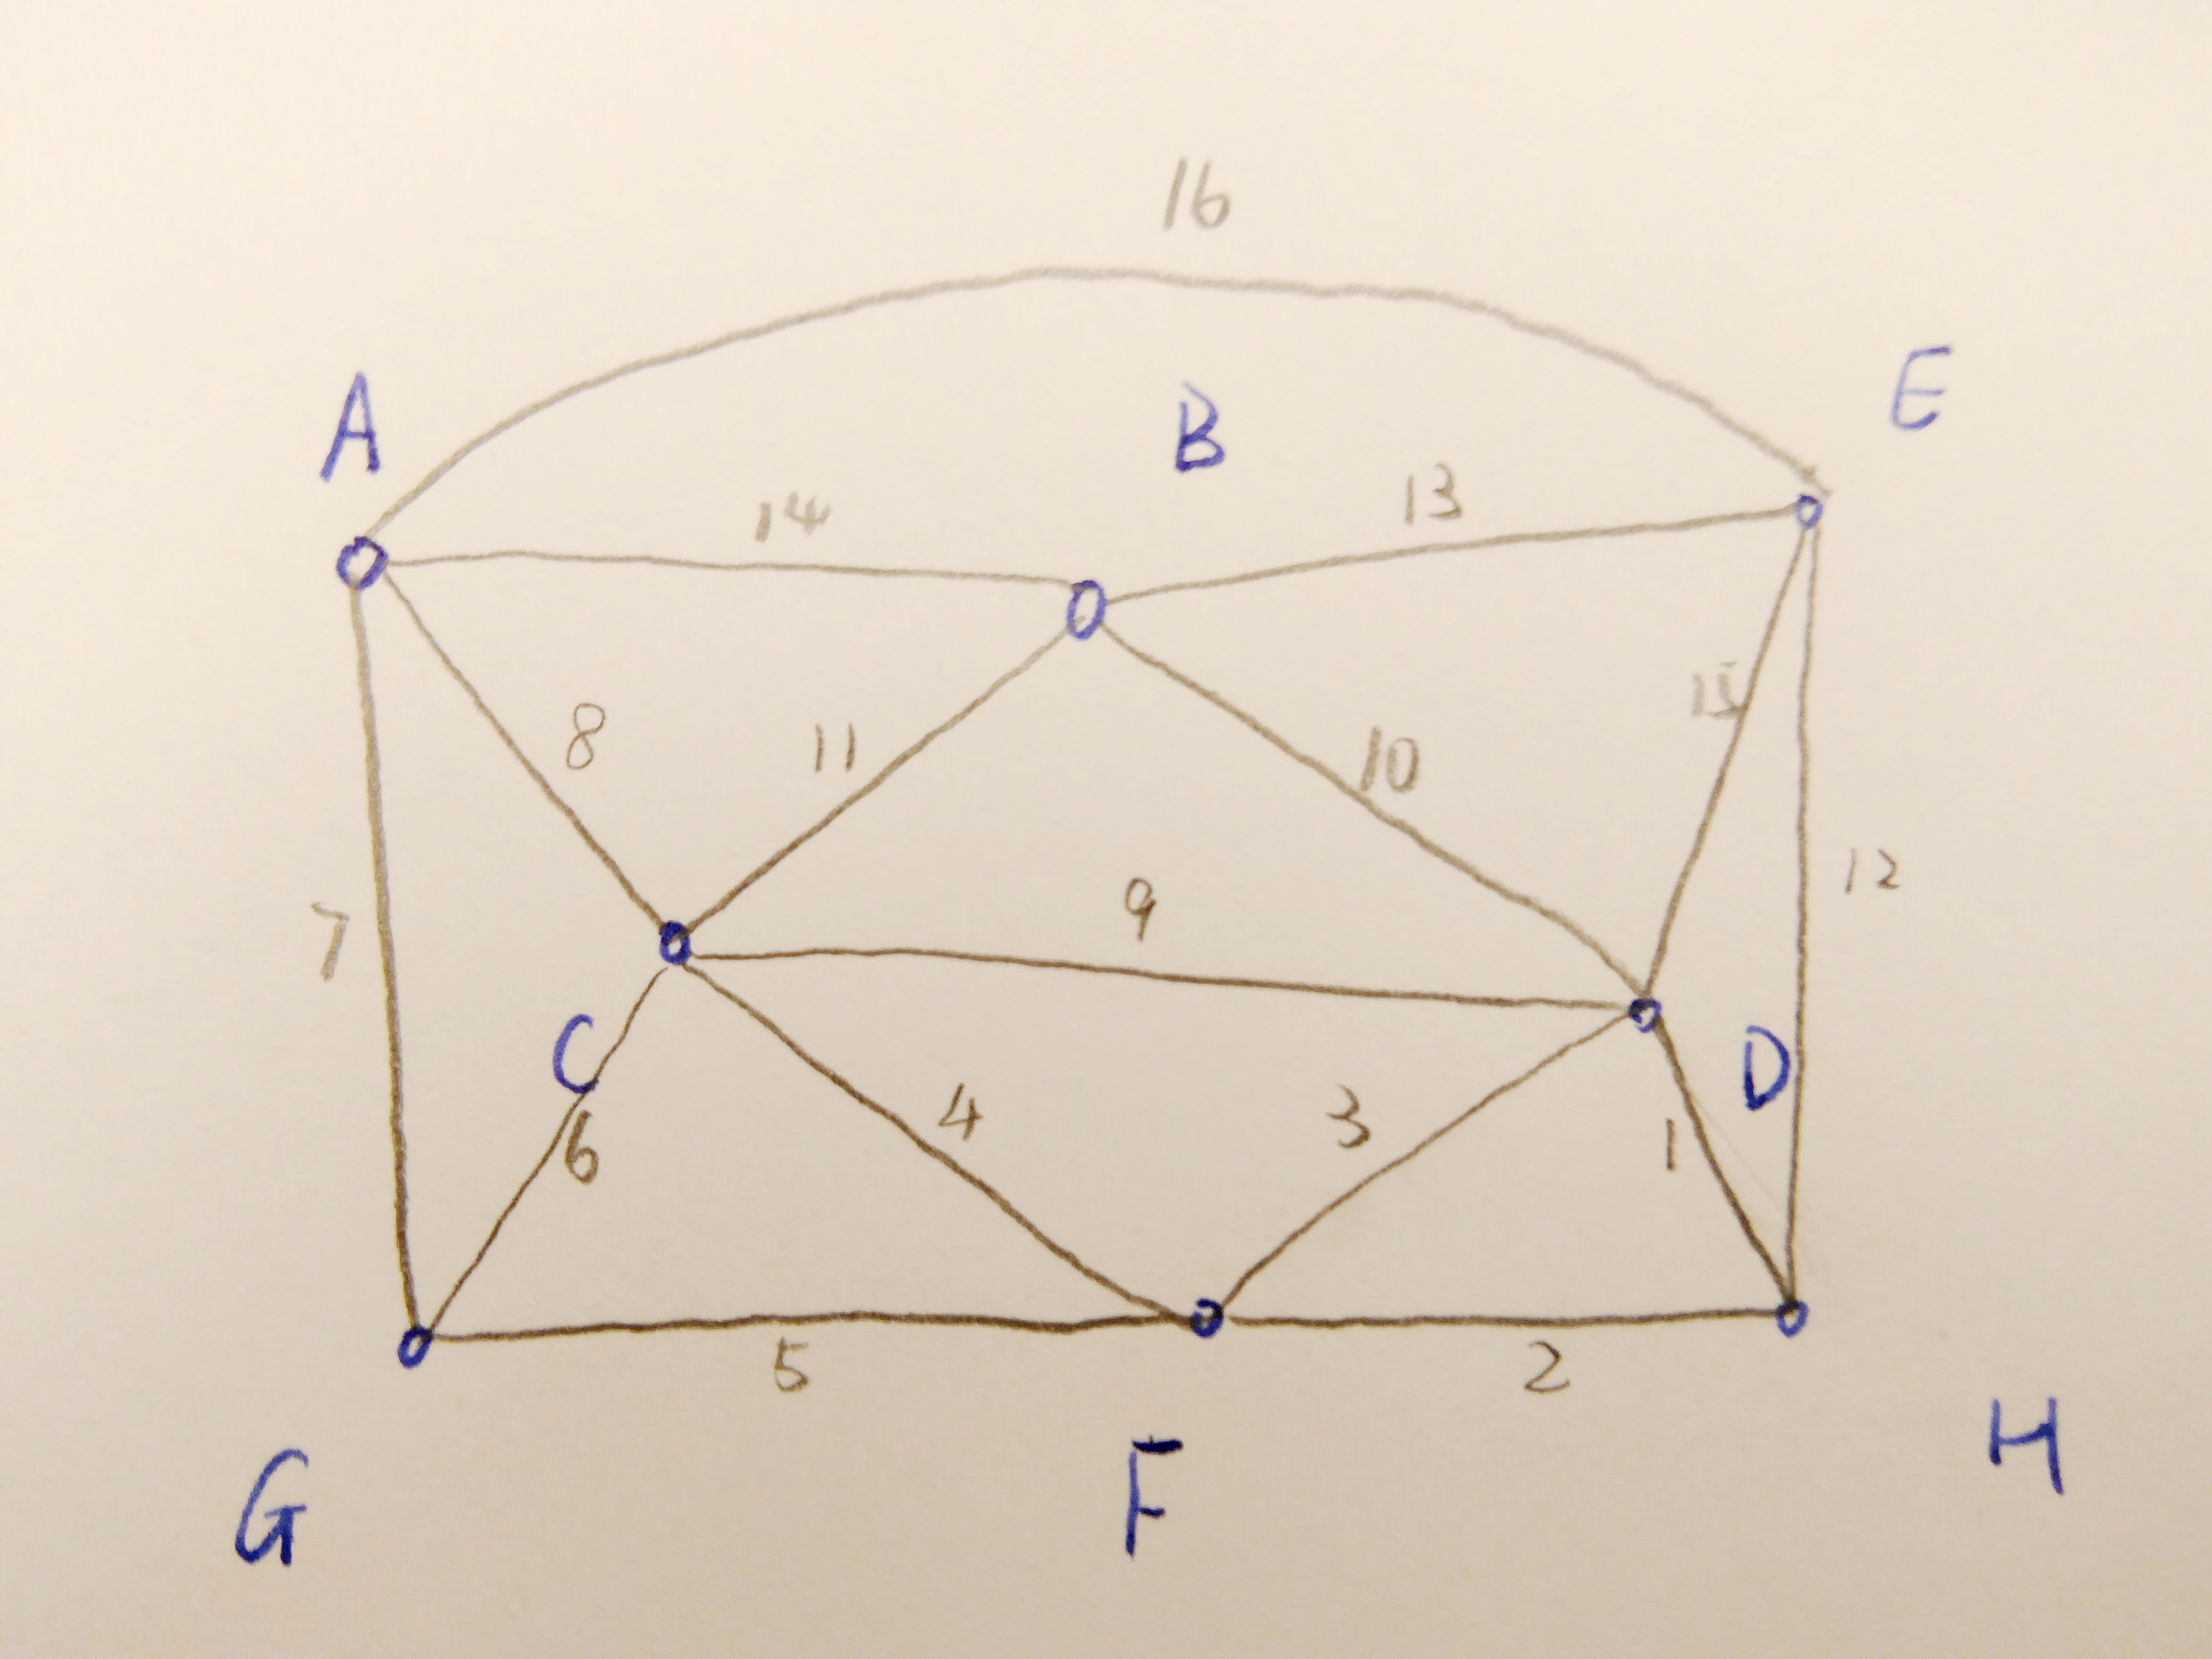
\includegraphics[width=0.75\linewidth]{Figure/1a1.jpg}
		\caption{Initial Figure}
		\label{fig:subfig1:a}
	\end{minipage}
	\begin{minipage}[t]{0.50\linewidth}
		\centering
		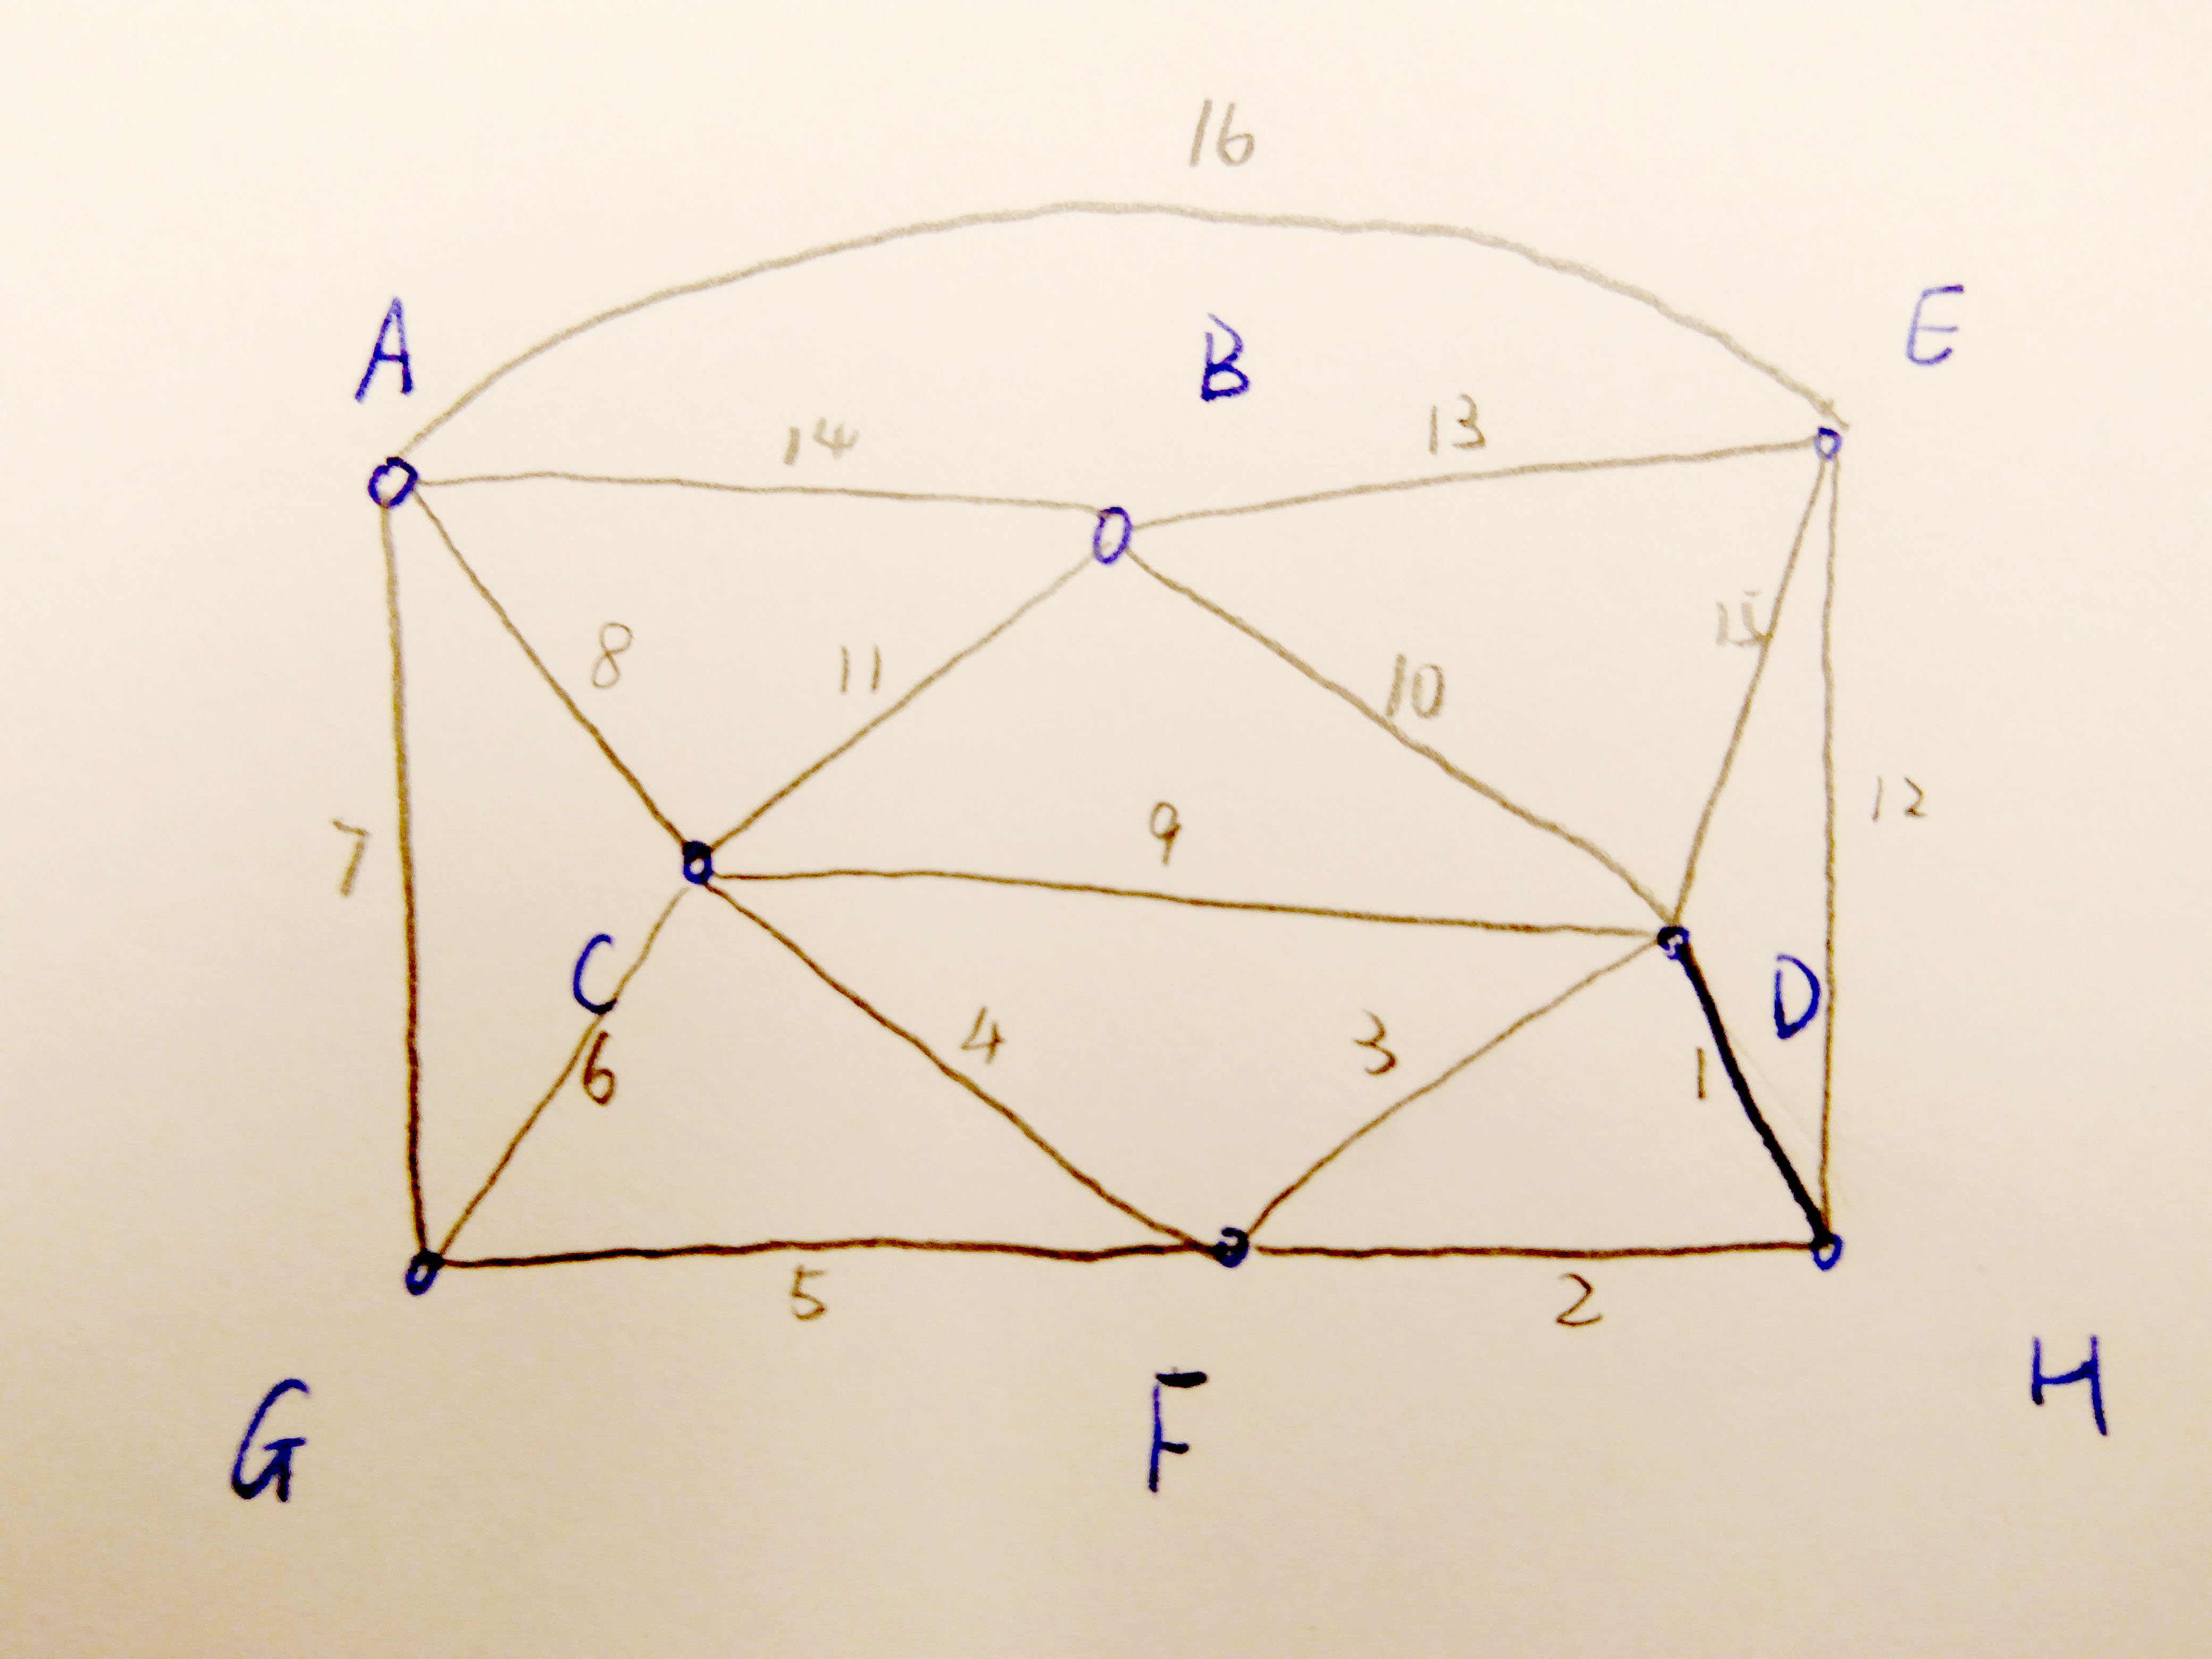
\includegraphics[width=0.75\linewidth]{Figure/1a2.jpg}
		\caption{Add $(D,H)$ to the tree}
		\label{fig:subfig1:b}
	\end{minipage}
\\
	\begin{minipage}[t]{0.50\linewidth}
		\centering
		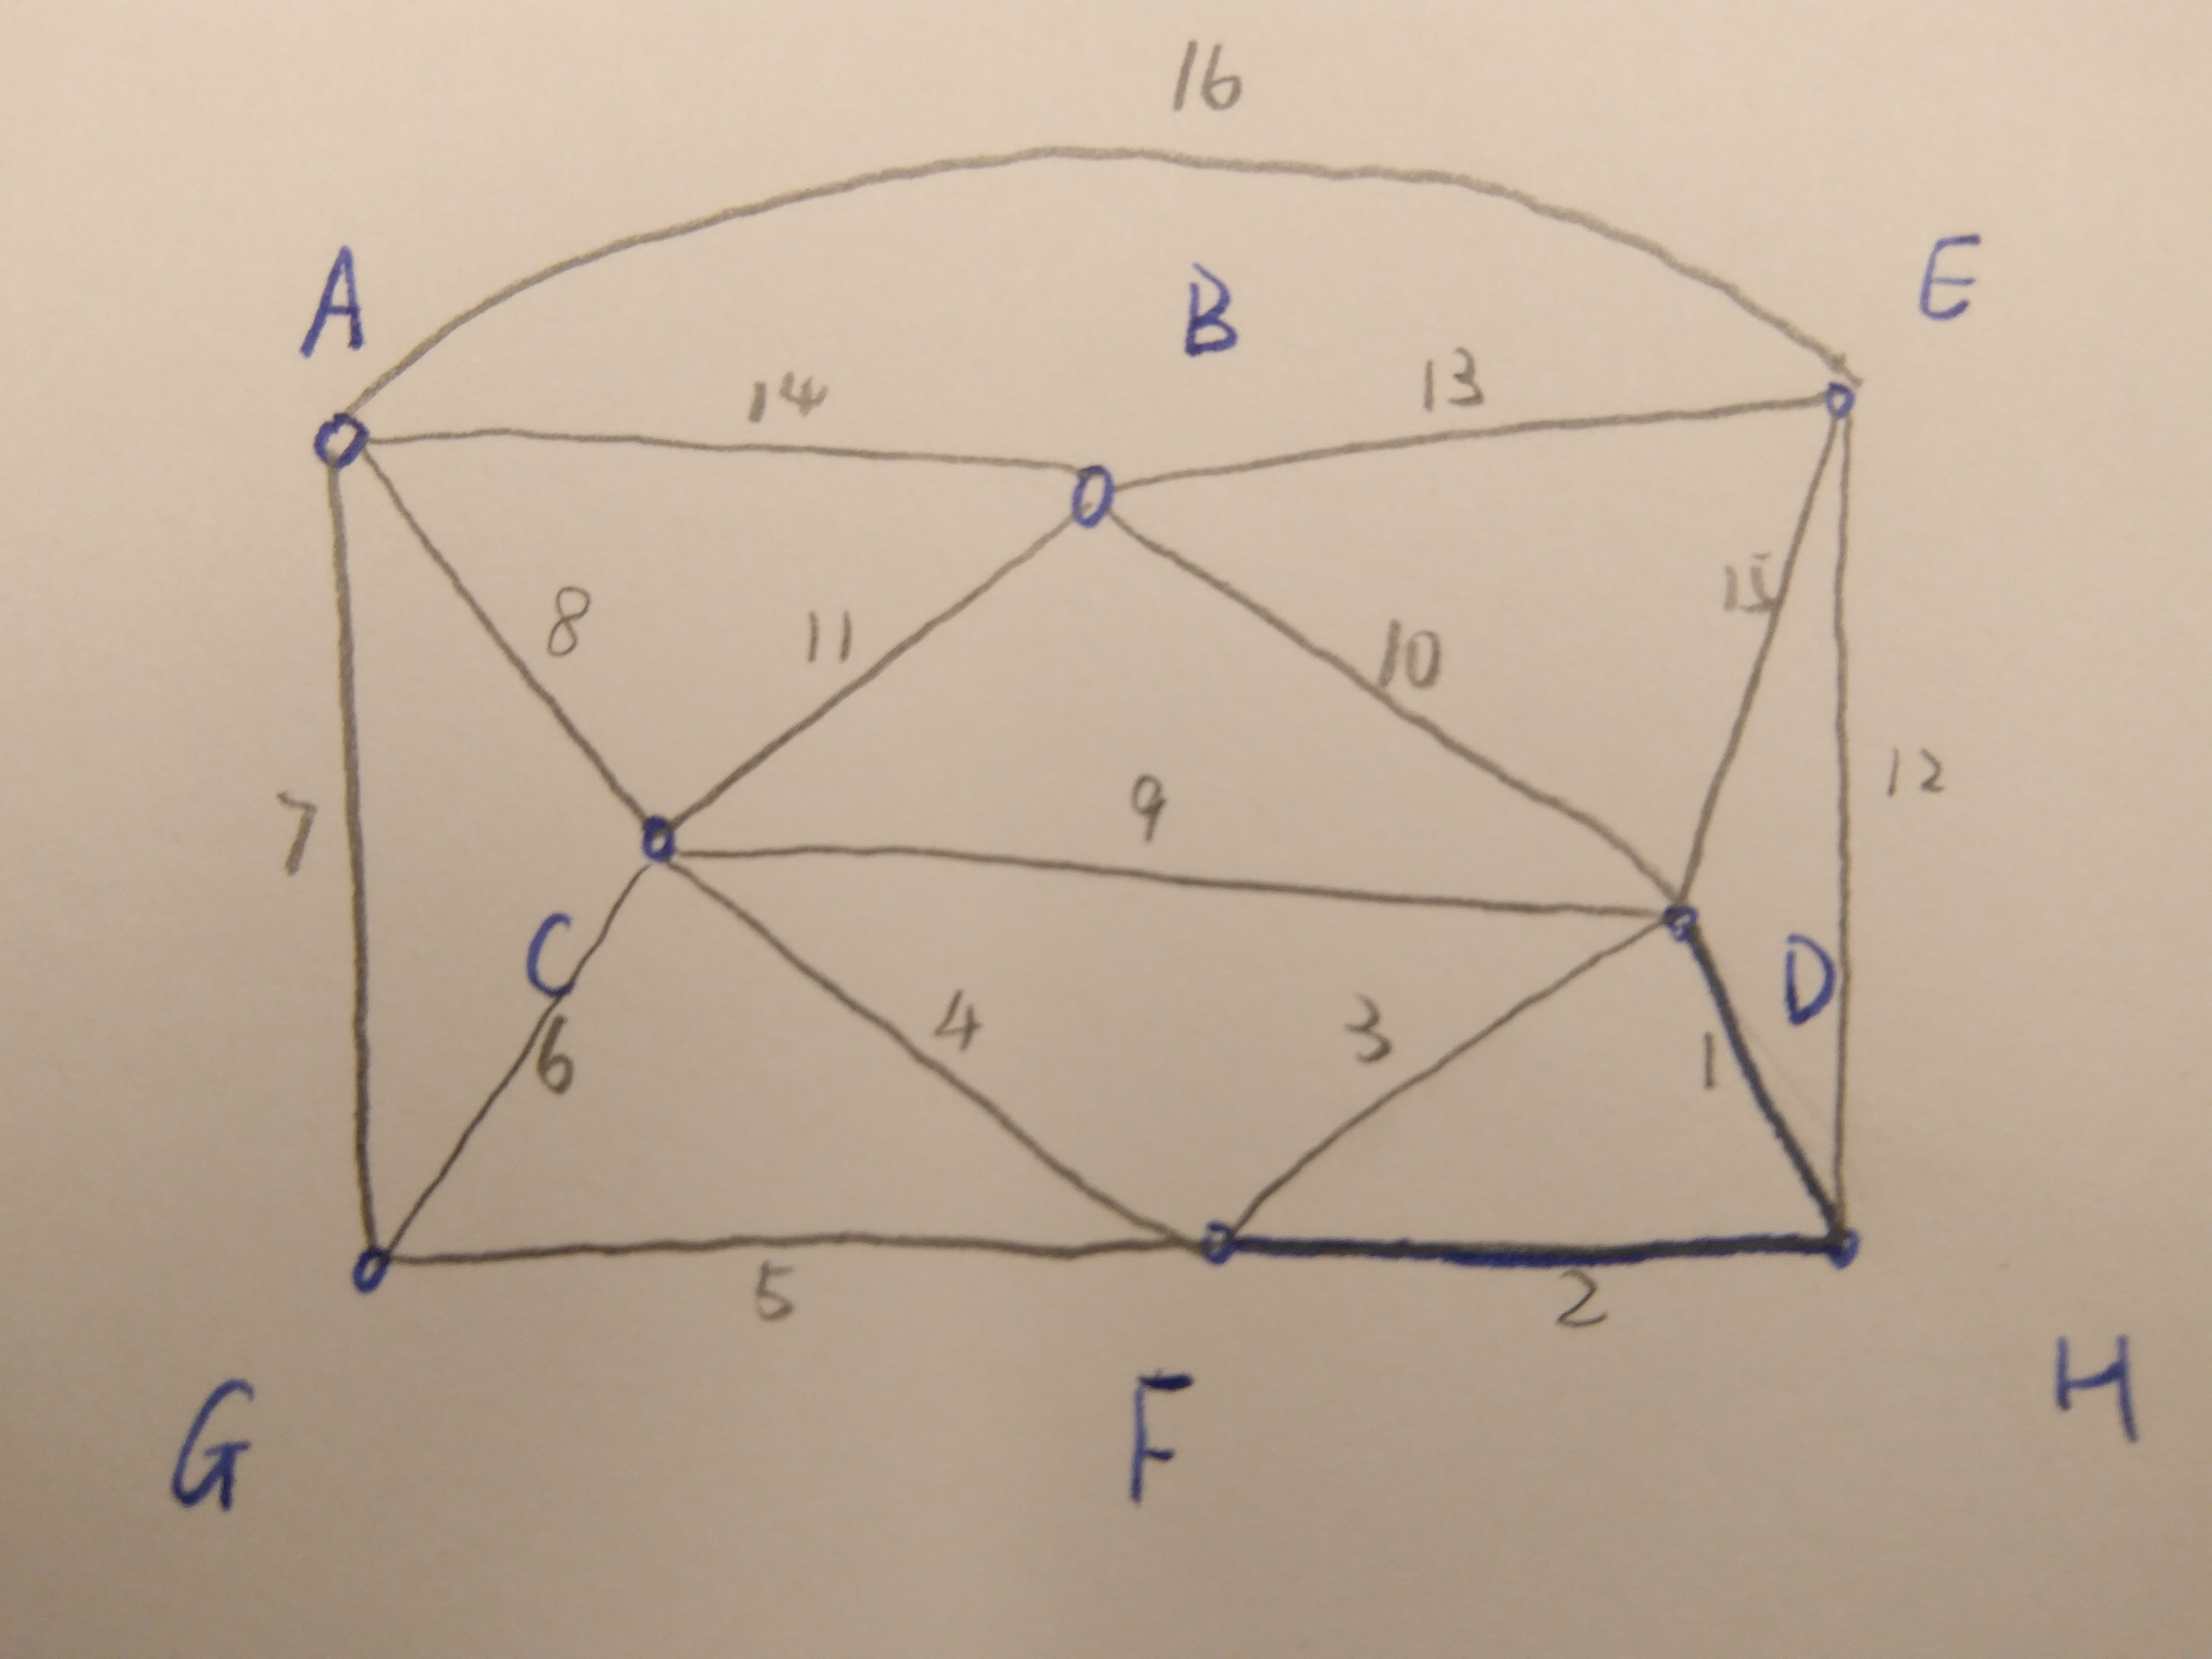
\includegraphics[width=0.75\linewidth]{Figure/1a3.jpg}
		\caption{Add $(F,H)$ to the tree}
		\label{fig:subfig1:c}
	\end{minipage}
	\begin{minipage}[t]{0.50\linewidth}
		\centering
		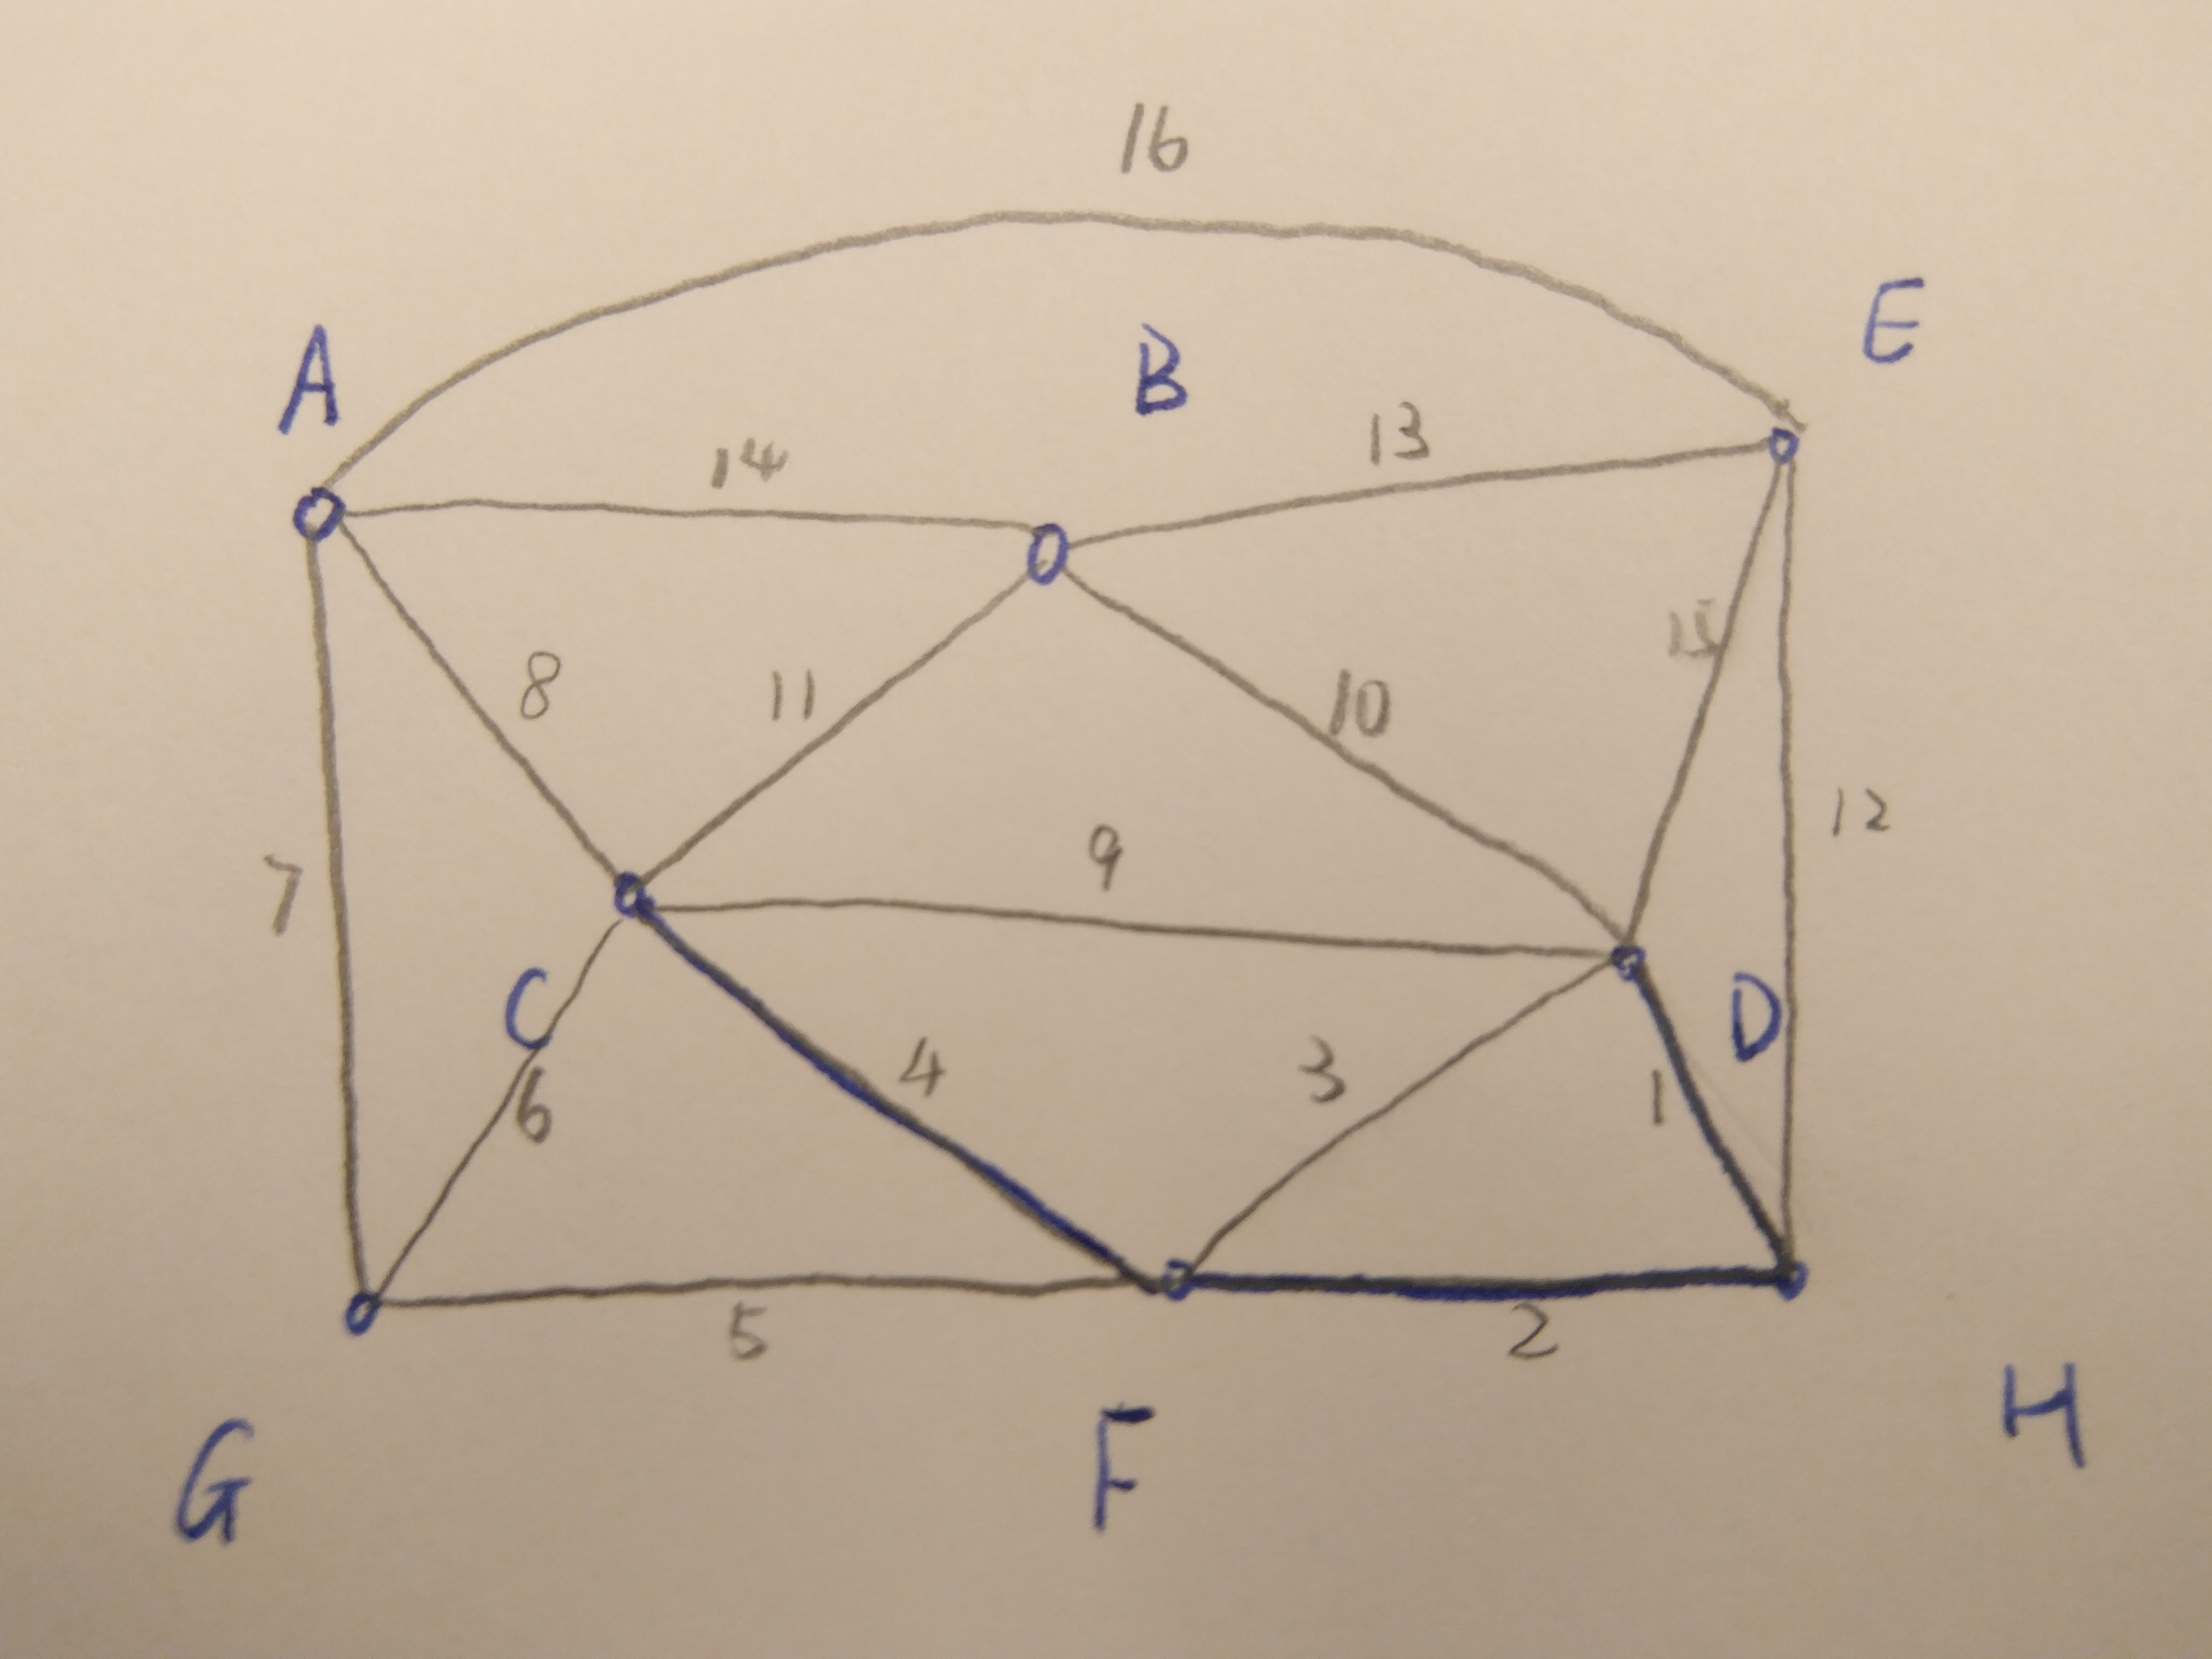
\includegraphics[width=0.75\linewidth]{Figure/1a4.jpg}
		\caption{Add $(C,F)$ to the tree}
		\label{fig:subfig1:d}
	\end{minipage}
\\
	\begin{minipage}[t]{0.50\linewidth}
		\centering
		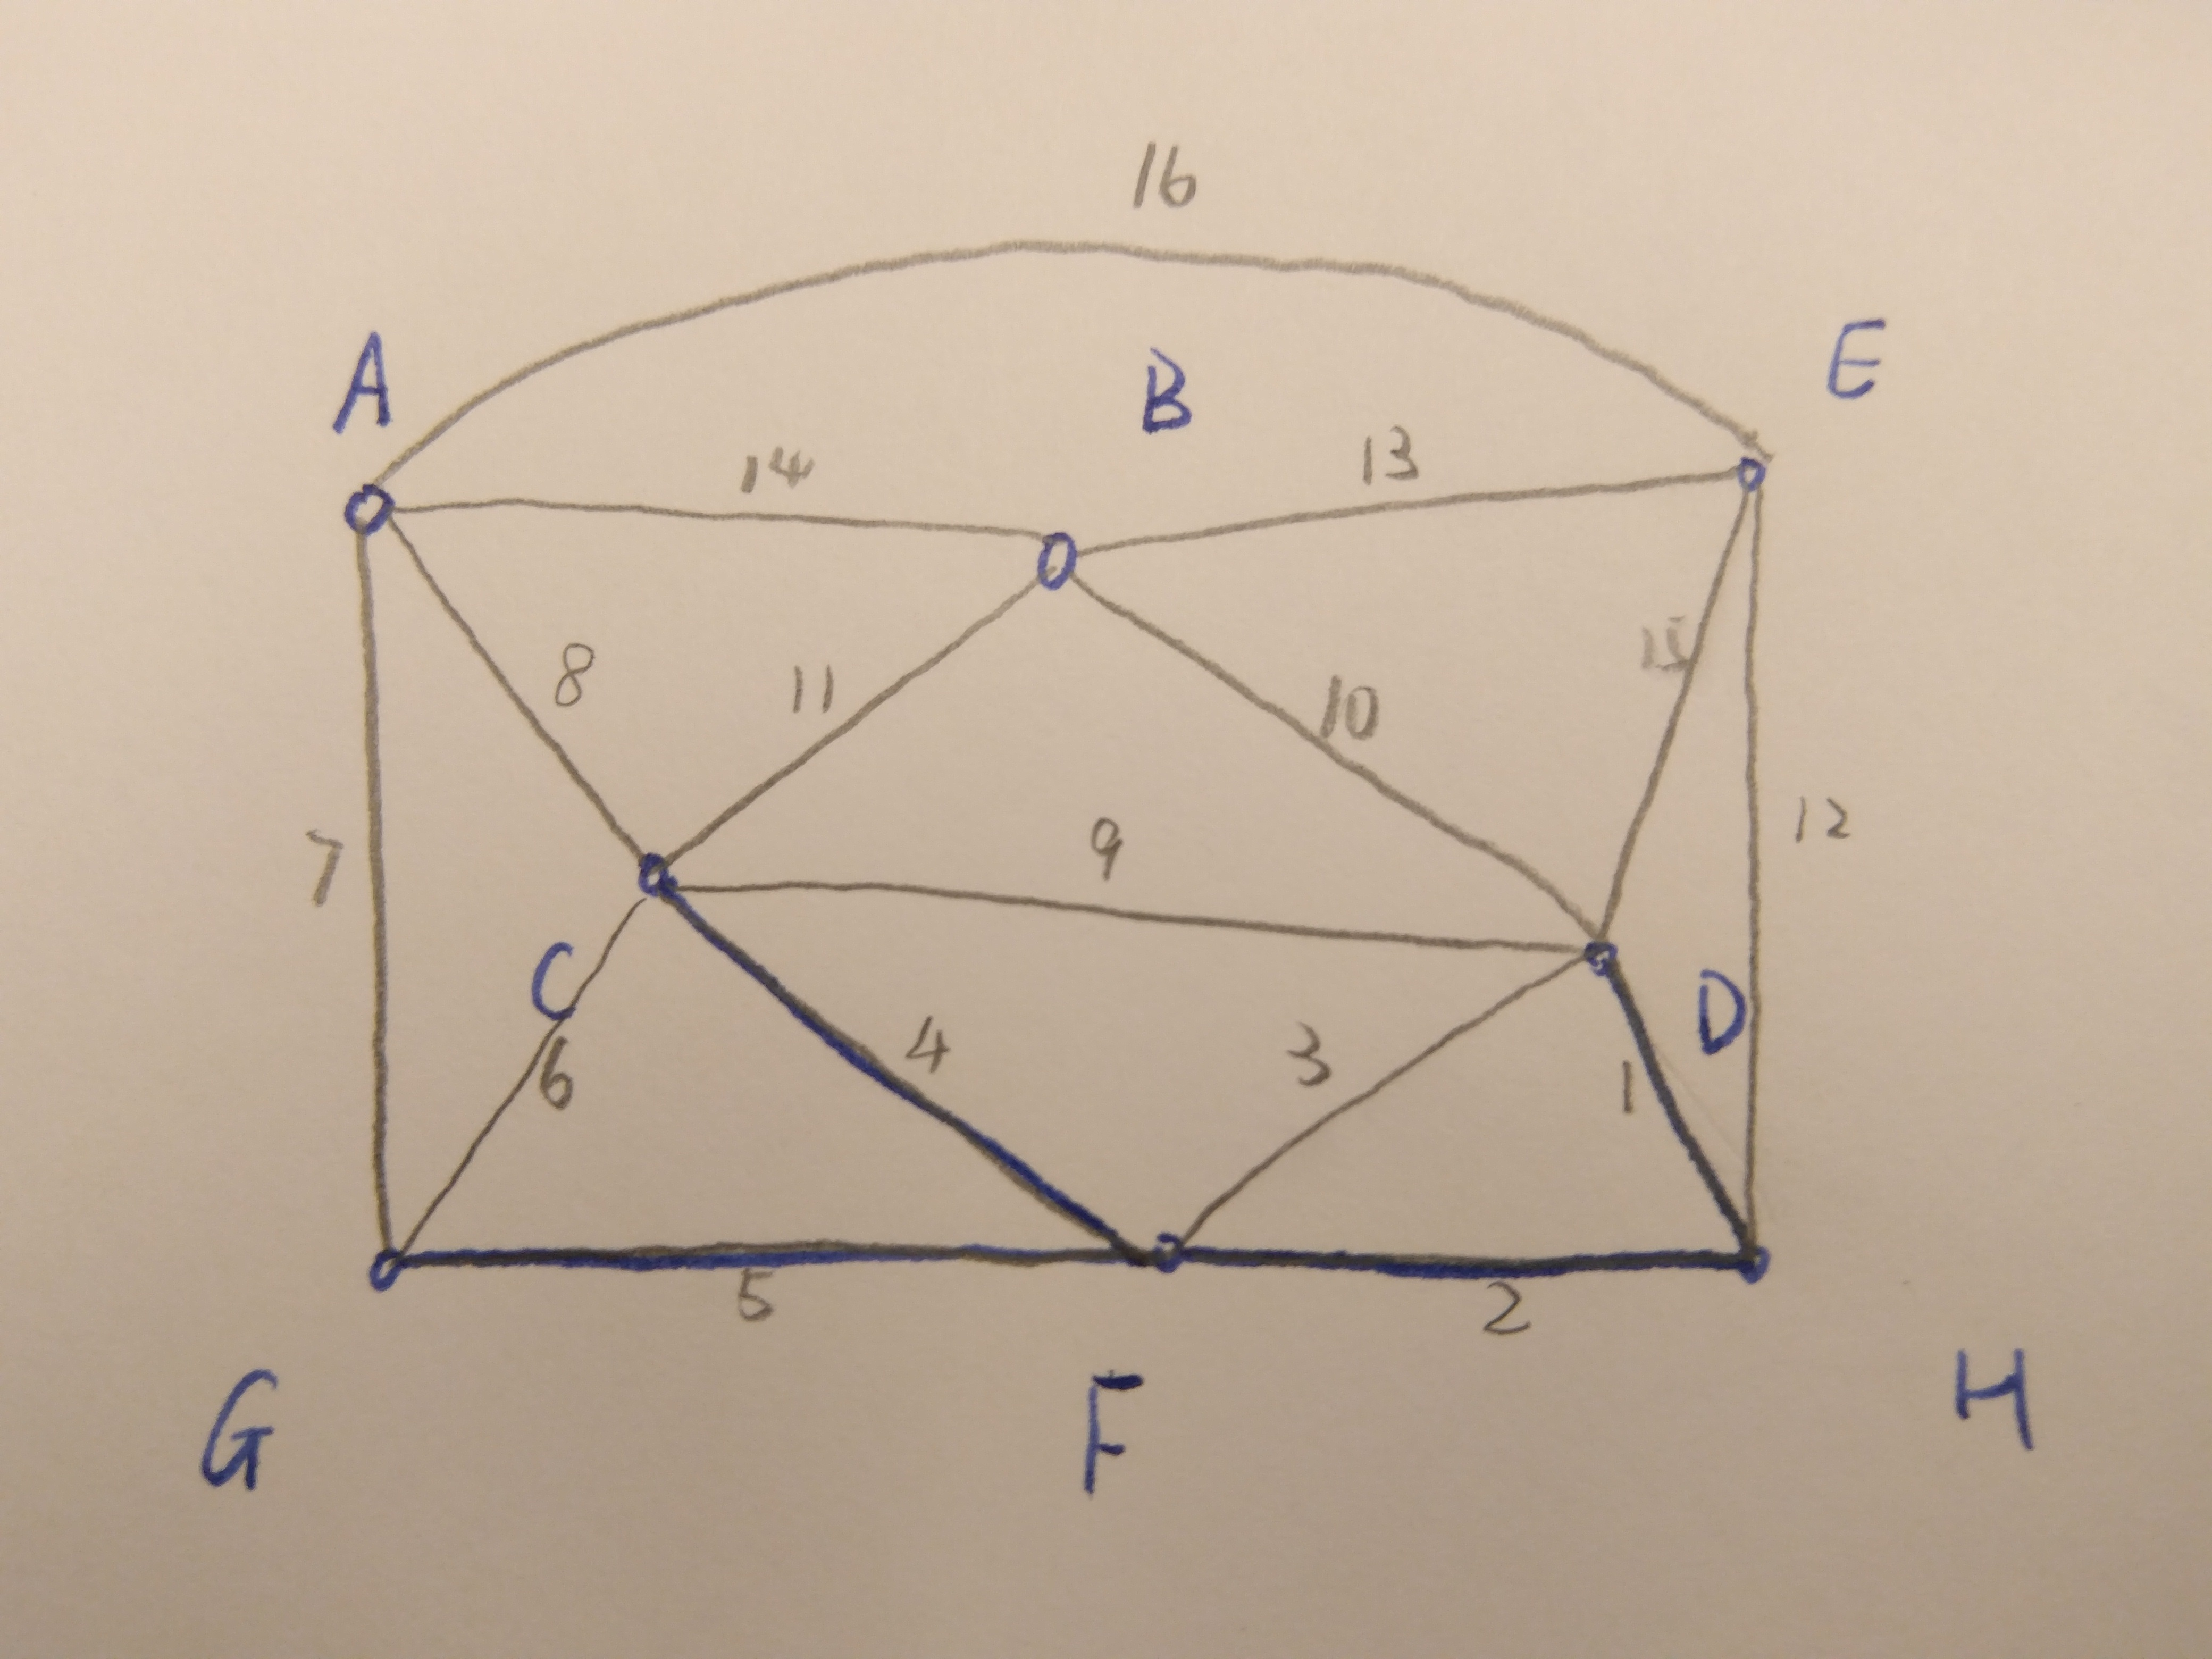
\includegraphics[width=0.75\linewidth]{Figure/1a5.jpg}
		\caption{Add $(G,H)$ to the tree}
		\label{fig:subfig1:e}
	\end{minipage}
	\begin{minipage}[t]{0.50\linewidth}
		\centering
		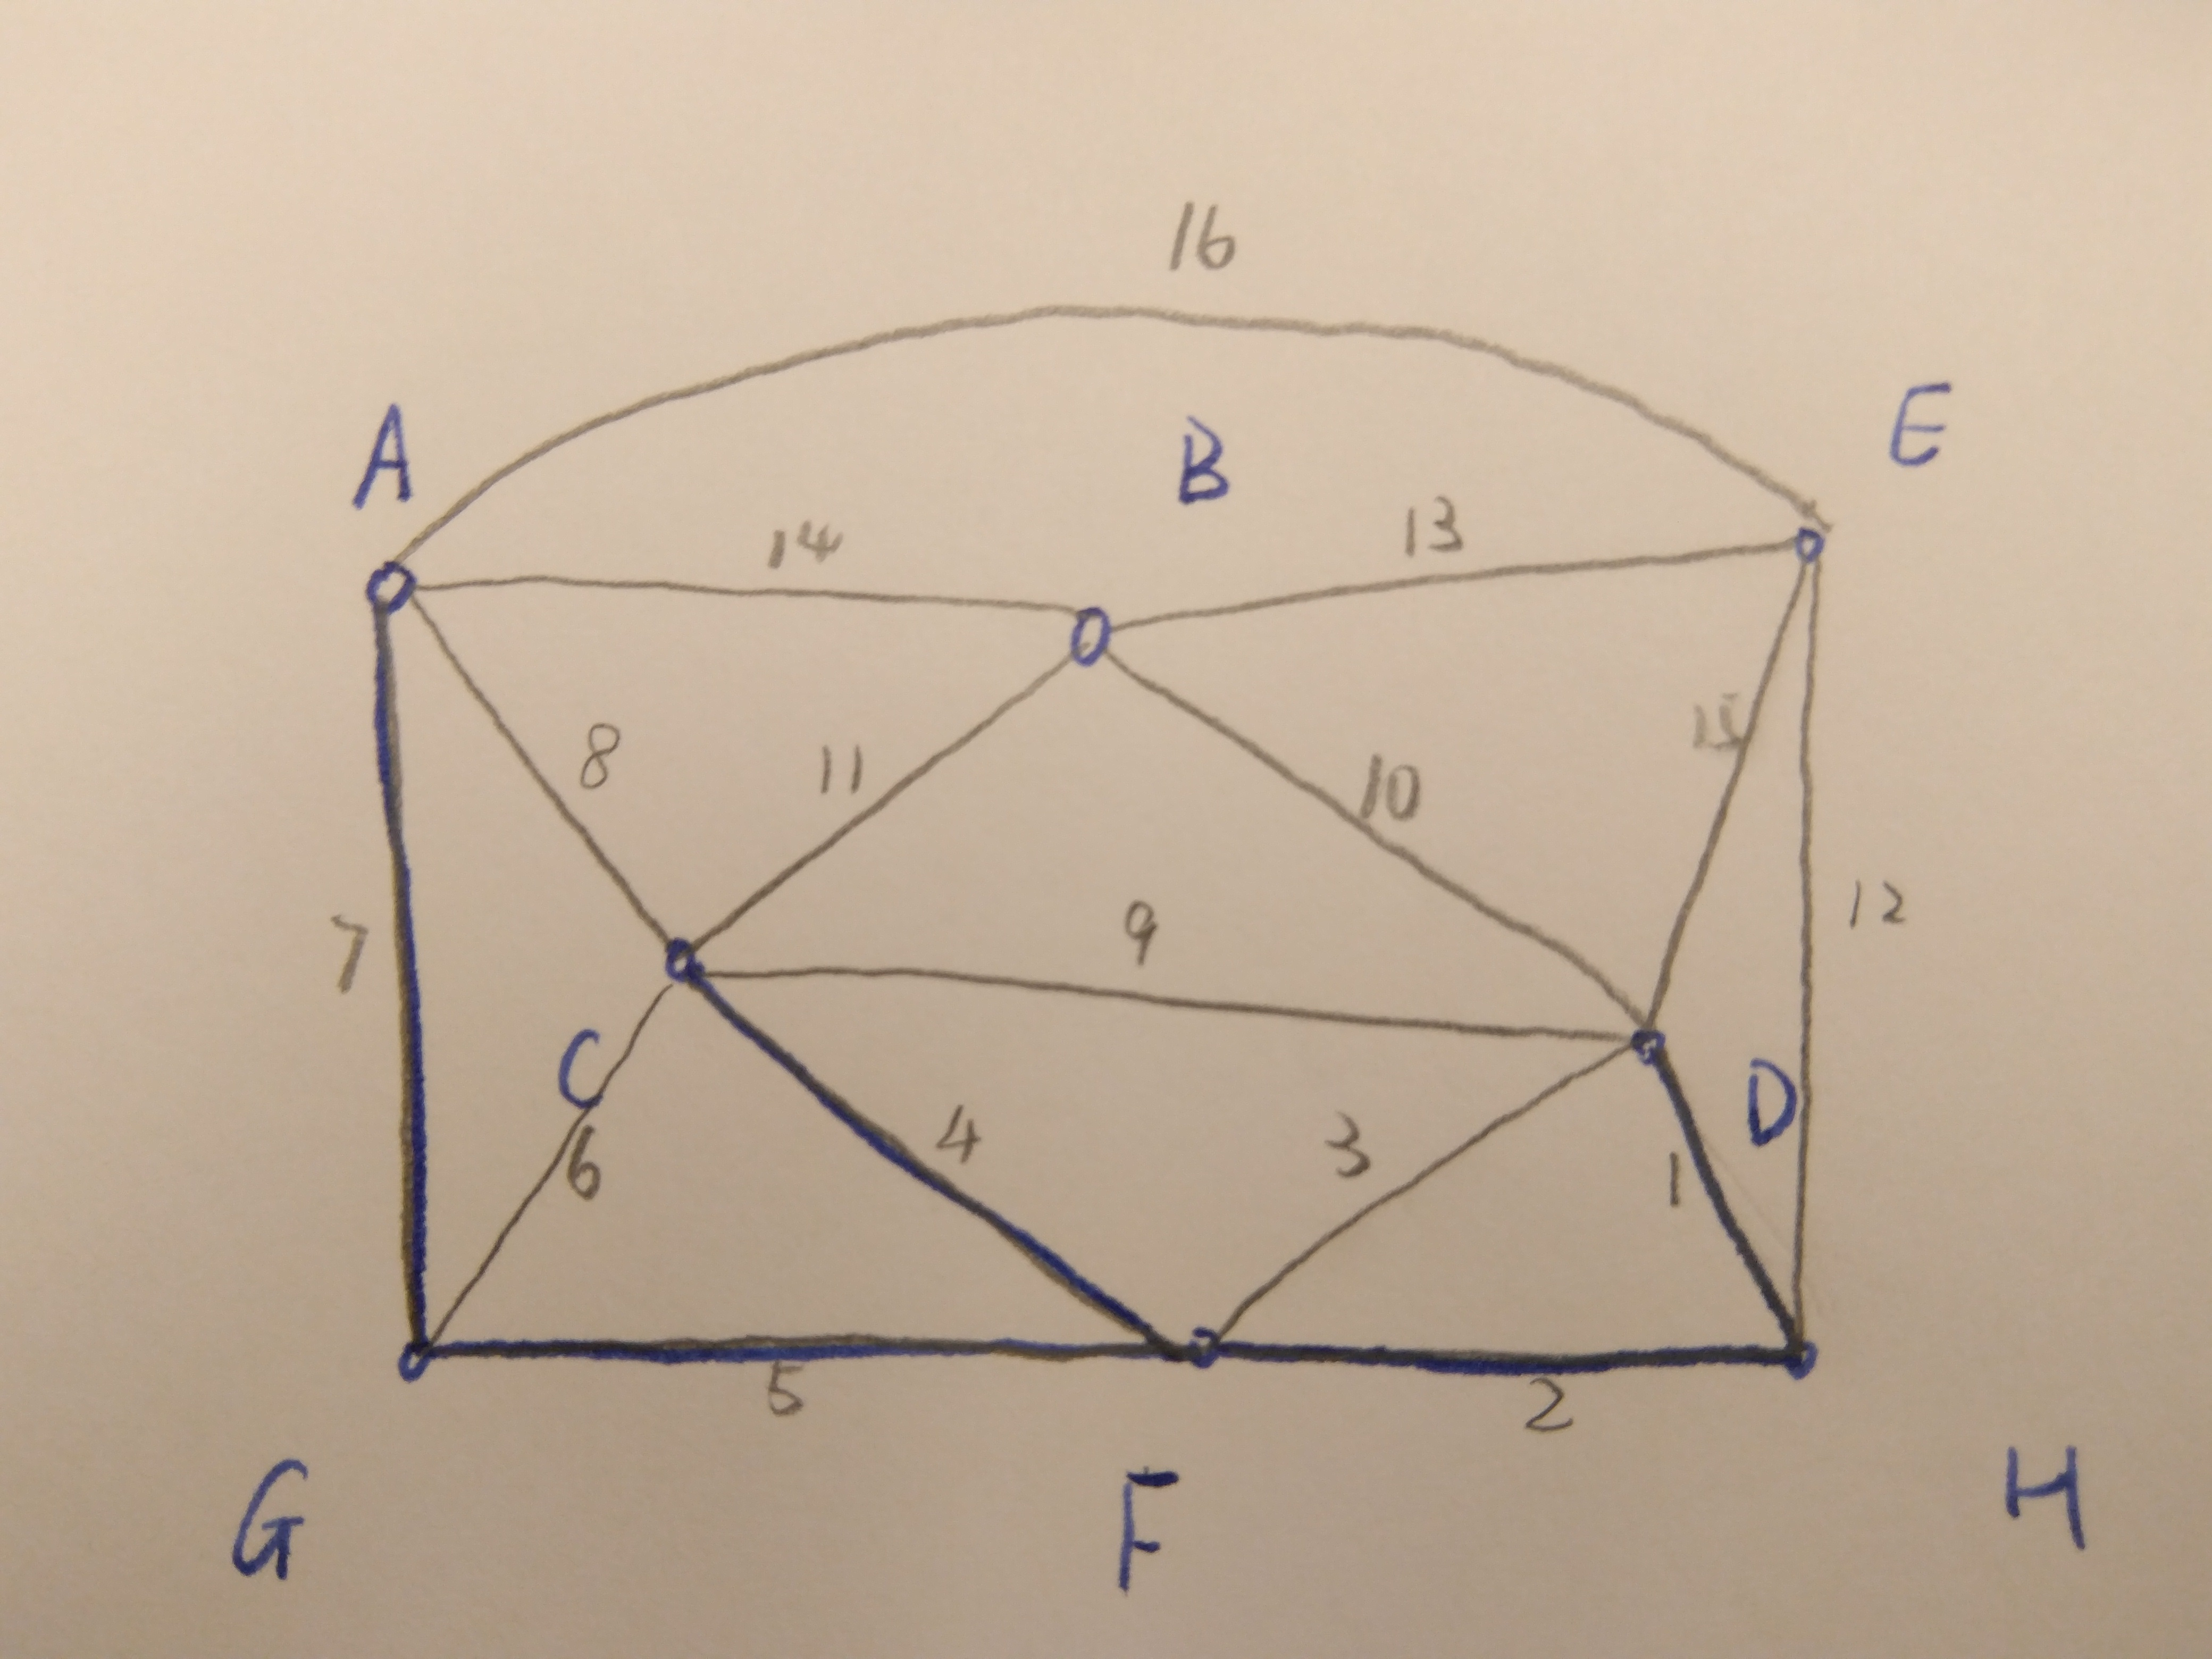
\includegraphics[width=0.75\linewidth]{Figure/1a6.jpg}
		\caption{Add $(A,G)$ to the tree}
		\label{fig:subfig1:f}
	\end{minipage}
\\
	\begin{minipage}[t]{0.50\linewidth}
		\centering
		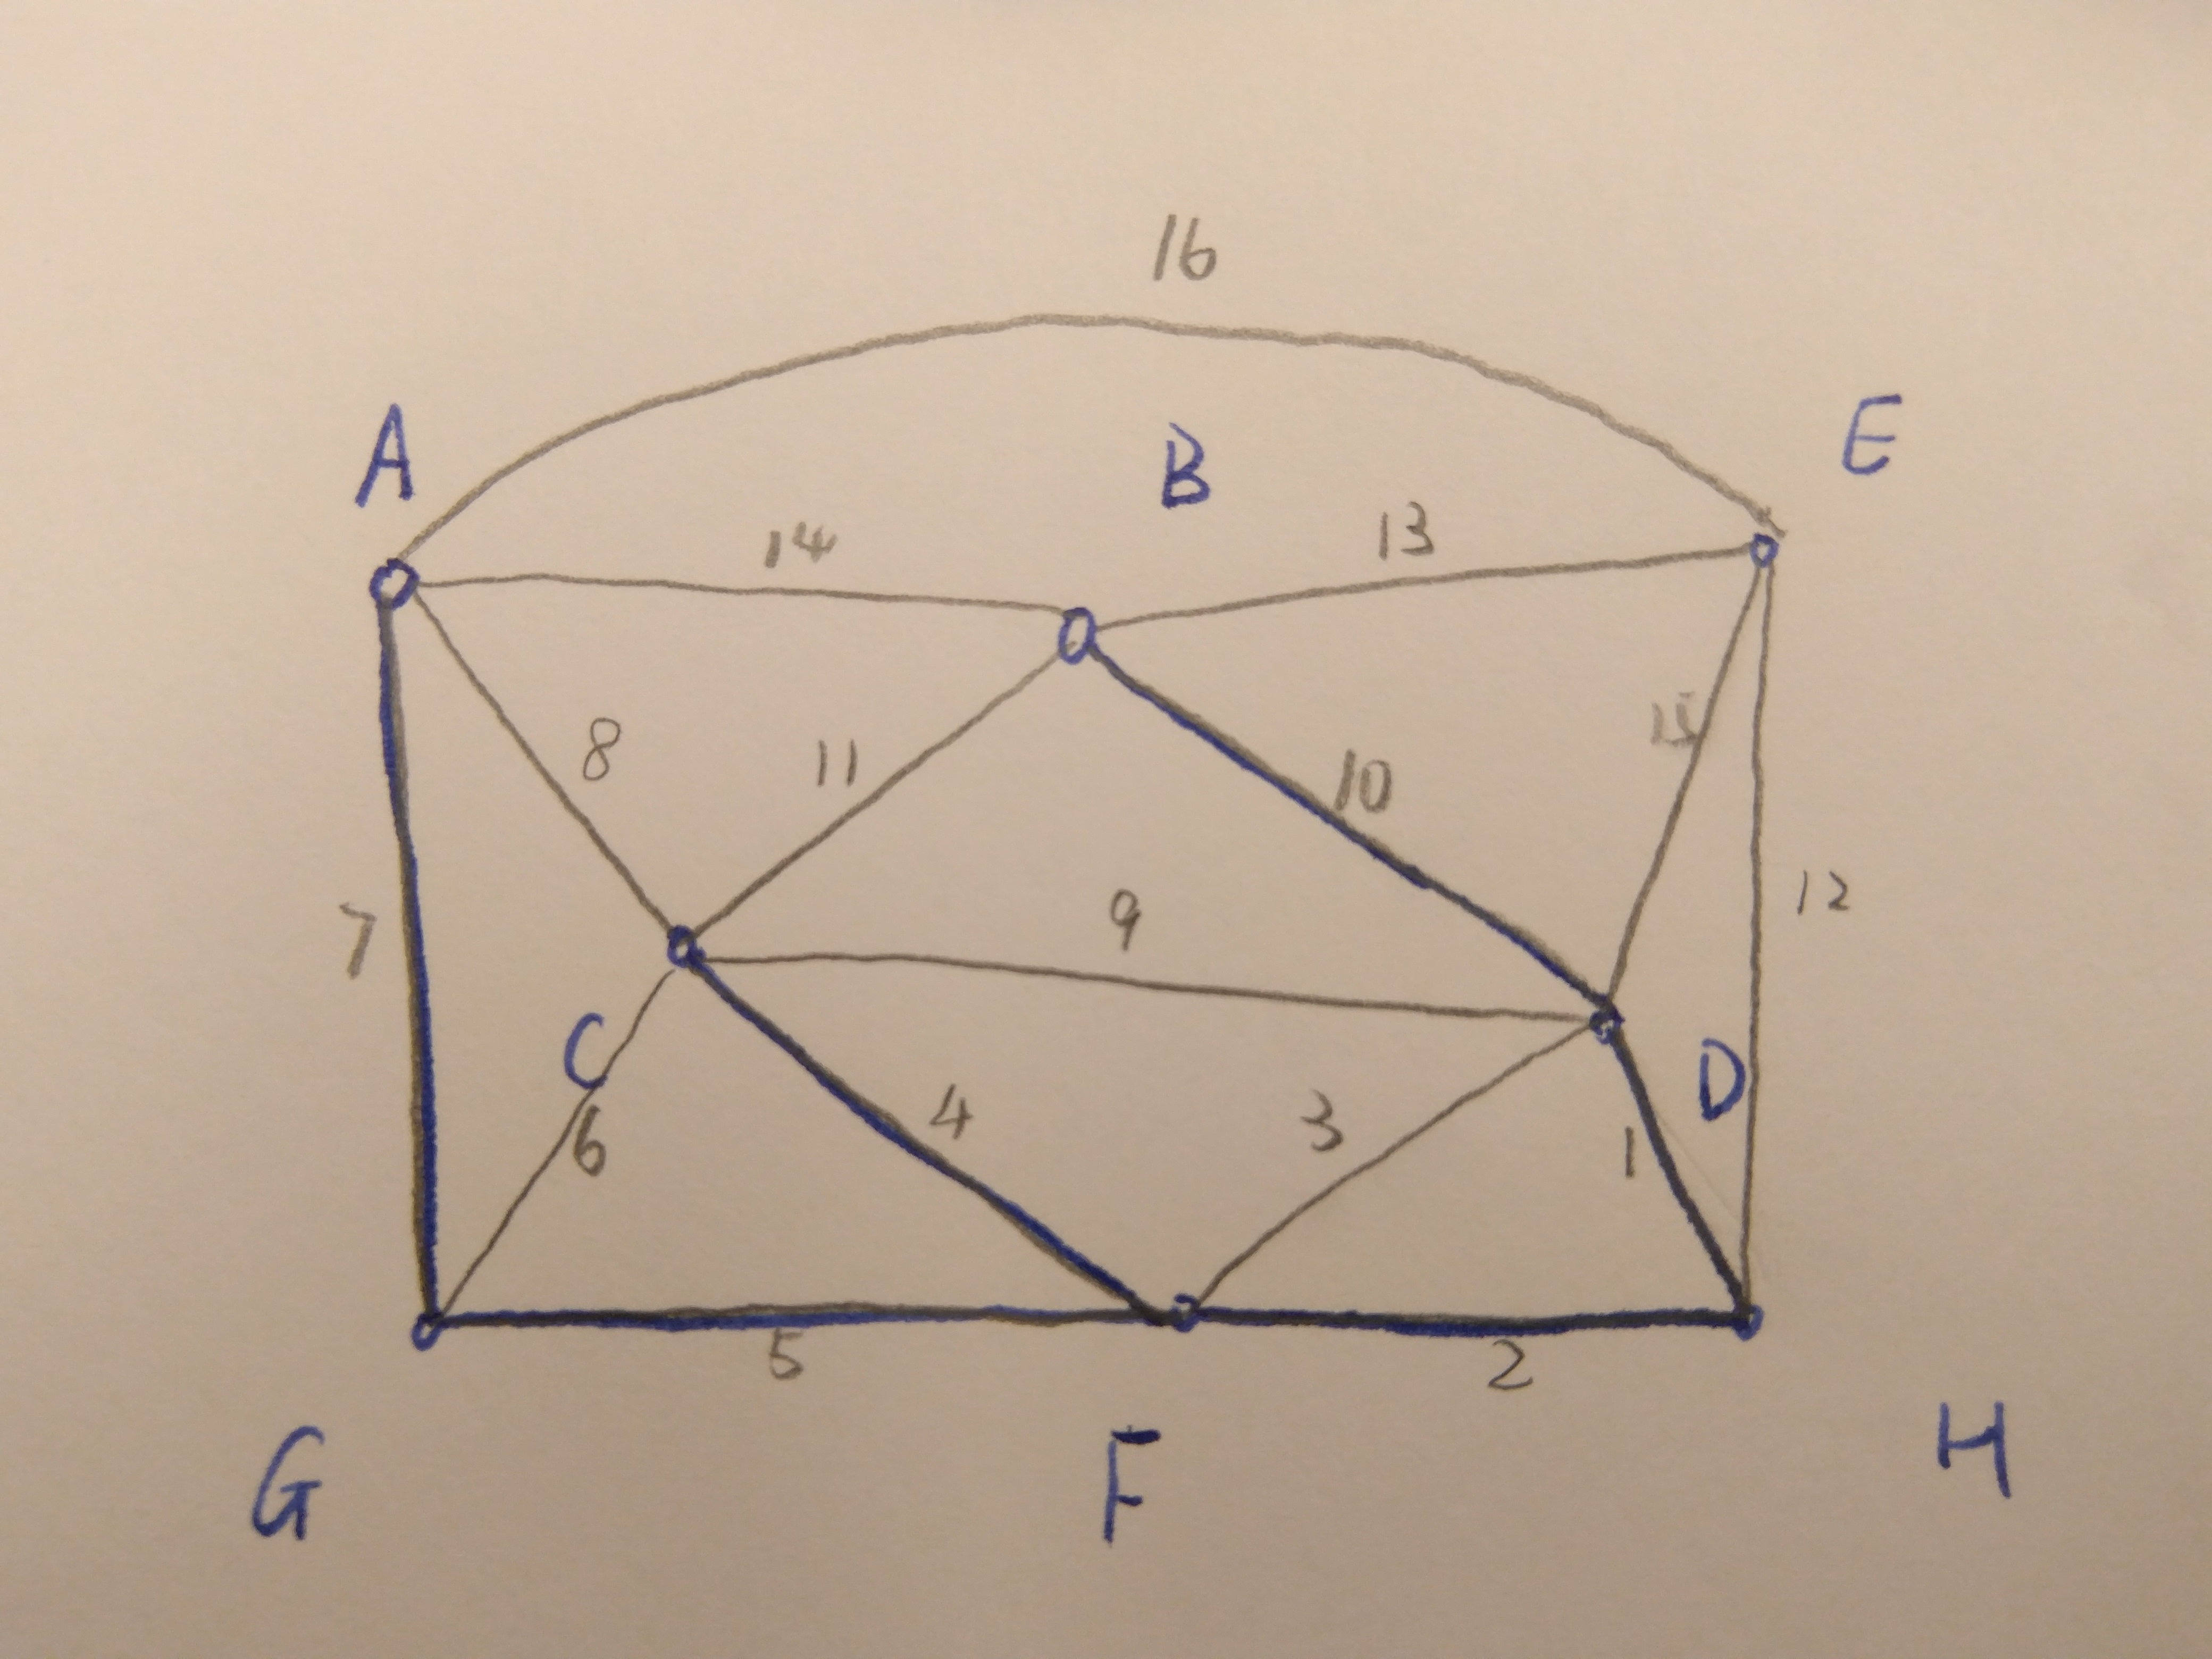
\includegraphics[width=0.75\linewidth]{Figure/1a7.jpg}
		\caption{Add $(B,D)$ to the tree}
		\label{fig:subfig1:g}
	\end{minipage}
	\begin{minipage}[t]{0.50\linewidth}
		\centering
		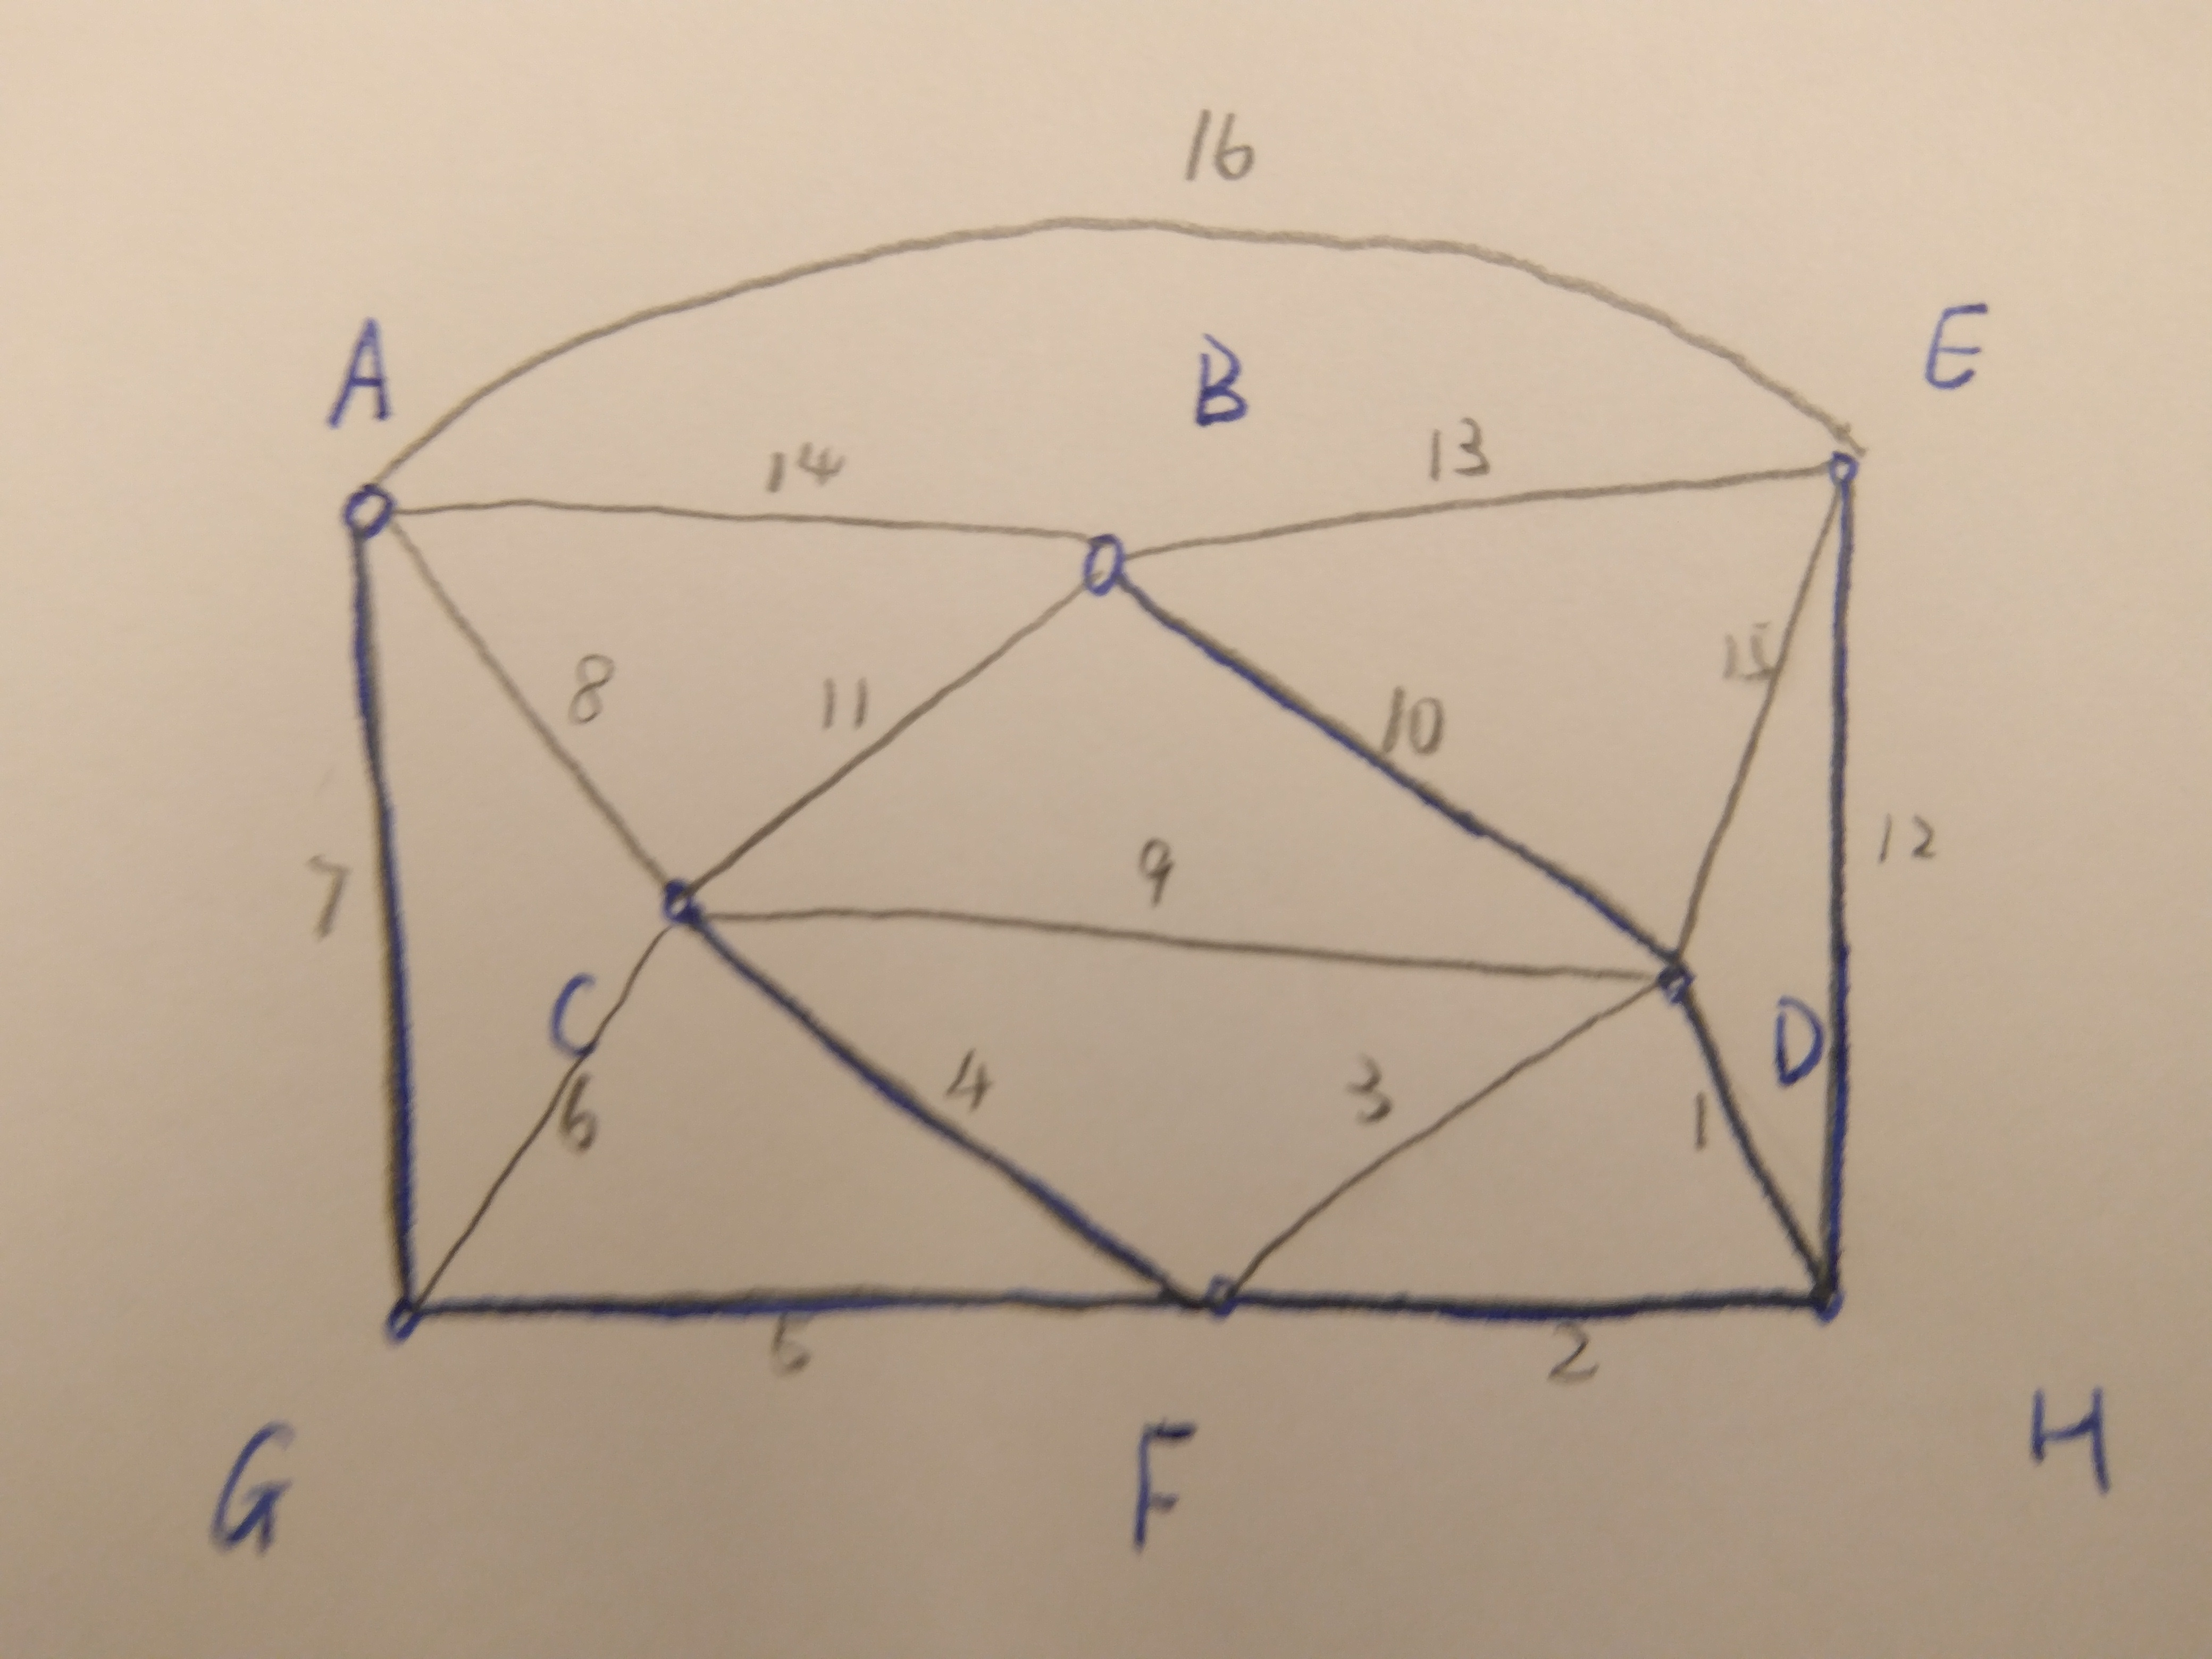
\includegraphics[width=0.75\linewidth]{Figure/1a8.jpg}
		\caption{Add $(E,H)$ to the tree}
		\label{fig:subfig1:h}
	\end{minipage}
\end{figure}
\subsection{R-18.3}
Give an example of a graph $G$ with at least $10$ vertices such that the greedy 2-approximation algorithm for VERTEX-COVER given above is guaranteed to produce a suboptimal vertex cover.

\noindent \textbf{\emph{Answer}}:
\section{Dijkstra Revisited}

\end{document}